\chapter{Physical implementation}\label{ch:implementation}

The implementation of the circuit was different in two ways compared to the original design:
\begin{itemize}
   \item \SI{120}{\kilo\ohm} resistors were used instead of \SI{100}{\kilo\ohm}, as they were easier to obtain, and would only result in a
         slightly larger gain and lower cutoff.
   \item The amplifier circuit was powered with regulated \SI{3.3}{V}. This was done to protect the ESP's input pins by saturating the output
         when it would have been too large.
\end{itemize}

\begin{figure}[!htb]
  \centering
  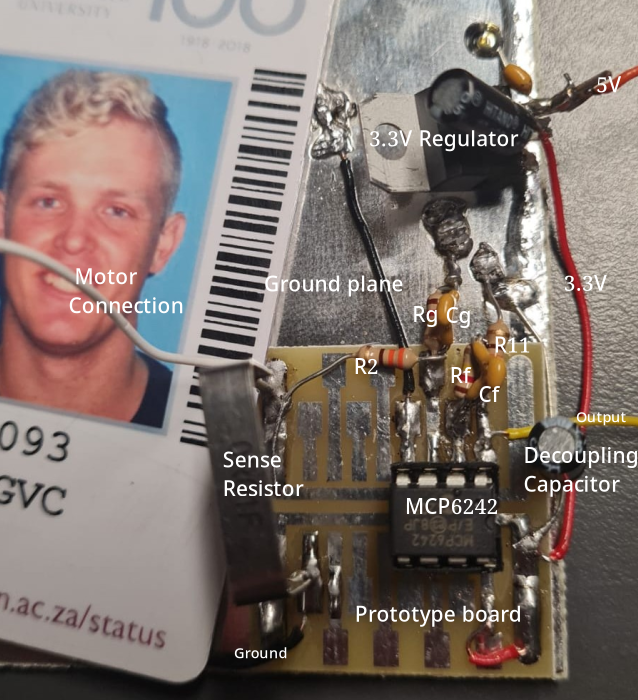
\includegraphics[width=0.8\textwidth]{Figures/physical_circuit}
  \caption{Final Circuit Implementation}
\end{figure}